\begin{frame}
\begin{columns}[t]
\begin{column}{0.5\textwidth}
\begin{block}{construction of $L$}
In order to construct the functor $L$, we need to explain the relationship between
\begin{itemize}
\item objects in the category of presheaves 
\item the {\it representable functors} from their underlying category
\end{itemize}
\end{block}
\end{column}
\begin{column}{0.5\textwidth}
%\centering\noindent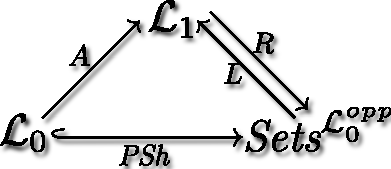
\includegraphics[width=1\columnwidth]{fig/ascent.pdf}
\begin{block}{Yoneda extension}
$$
\xymatrix{
& \mathcal{L}_1 & \\
\mathcal{L}_0 \ar[ru]^{A} \ar[rr]_{PSh} & & \textit{Sets}^{\mathcal{L}_0^{opp}} \ar@{-->}[lu]_{L}
}
$$
\end{block}
\end{column}
\end{columns}
\end{frame}